\chapter{Estado del arte}

\section{Chatbots}

Un chatbot o agente conversacional\textit{(\cite{chatbots2020})} es un programa inteligente que mediante lenguaje escrito u oral pueden interactuar con los usuarios a través de una conversación de lenguaje natural. 

La Inteligencia Artificial se integra cada vez más nuestra vida cotidiana con la creación y el análisis de software y hardware inteligentes, llamados agentes inteligentes. Los agentes inteligentes pueden realizar una gran variedad de tareas, desde trabajos manuales hasta operaciones sofisticadas. Un chatbot es un ejemplo típico de sistema de IA y uno de los ejemplos más elementales y extendidos de Interacción Persona-Ordenador inteligente. Se trata de un programa informático que responde como una entidad inteligente cuando se conversa con él a través de texto o voz y que entiende uno o más lenguajes humanos mediante el Procesamiento del Lenguaje Natural (PLN). En el léxico, un chatbot se define como "Un programa informático diseñado para simular una conversación con usuarios humanos, especialmente a través de Internet".

En el ámbito empresarial los chatbots se han convertido en una forma cada vez más popular de que las empresas interactúen con sus clientes \textit{(\cite{techinnovation})}. Proporcionan una forma cómoda y eficaz de obtener respuestas a las consultas de los clientes, ayudarles a realizar compras e incluso ofrecerles recomendaciones personalizadas. Como resultado, cada vez más empresas están implementando chatbots en sus operaciones de atención al cliente. En este artículo, analizaremos las diversas formas en que las empresas están aprovechando la tecnología de chatbot para mejorar su experiencia de servicio al cliente y cómo se pueden utilizar también en otras áreas de negocio.

\begin{figure}[!ht]
    \centering
    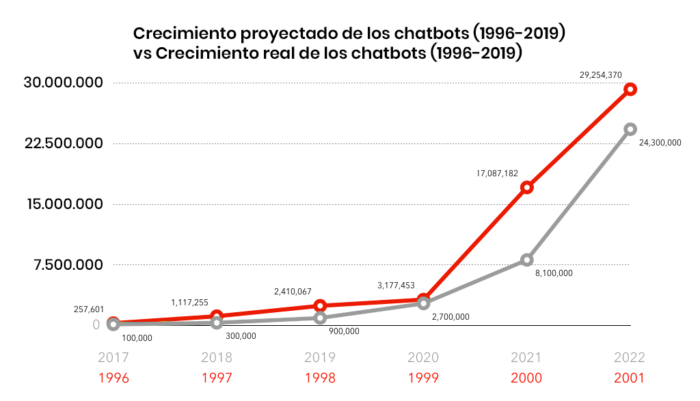
\includegraphics[width=1\textwidth]{imagenes/uso_chatbots.png}
    \caption{ Crecimiento del uso de chatbots en los últimos año \textit{(\cite{crecimientochatbots})} }
    \label{fig:enter-label}
\end{figure}

\subsection{Tipos de chatbots}

Un chatbot funciona de un par de maneras: con directrices establecidas y mediante aprendizaje automático (ML).{\vspace{0.3cm}

\textit{\textbf{Set Guidelines Chatbots}}: Un chatbot que funciona con un conjunto de directrices establecidas está limitado en su conversación. Sólo puede responder a un número determinado de peticiones y vocabulario y es tan inteligente como su código de programación. Un ejemplo de bot limitado es un bot bancario automatizado que hace algunas preguntas a la persona que llama para entender lo que quiere hacer.{\vspace{0.3cm}


\textit{\textbf{Machine Learning Chatbots}}: Un chatbot que funciona mediante aprendizaje automático tiene una red neuronal artificial inspirada en los nodos neuronales del cerebro humano. El bot está programado para autoaprender a medida que se le presentan nuevos diálogos y palabras. En efecto, a medida que un chatbot recibe nuevos diálogos de voz o textuales, aumenta el número de consultas a las que puede responder y la precisión de cada respuesta que da.


Los chatbots se utilizan en diferentes sectores y se crean con diferentes fines. Hay bots de venta al por menor diseñados para recoger y encargar la compra, bots meteorológicos que dan la previsión del tiempo del día o de la semana, y bots simplemente amistosos que simplemente hablan con la gente que necesita un amigo.

\subsection{Canales de comunicación}

Los canales de comunicación desempeñan un papel importante a la hora de ayudar a las marcas y a los clientes a conectarse entre sí para diversas formas de compromiso e interacciones. La elección del canal adecuado es vital para que nuestro chatbot proporcione una experiencia efectiva y eficiente en los usuarios. Algunos de los más usados son:\vspace{0.3cm}

\textbf{Sitio Web y App móvil}: Uno de los canales más populares es en el sitio web de la empresa o en algunos casos en la App que dispongan. El chatbot puede responder preguntas frecuentes de los clientes y proporcionar asistencia en tiempo real.\vspace{0.3cm}

\textbf{Facebook}: Otra forma es integrándolo el chatbot en una página de Facebook. A través de Facebook Messenger los clientes pueden recibir respuestas automáticas al momento. Además Facebook brinda la oportunidad de integrar el chatbot en tu página para que responda comentarios de tu muro de forma automática.\vspace{0.3cm}

\textbf{WhatsApp}: Creando una cuenta en WhatsApp Business API, el bot puede responder instantáneamente al usuario y segmentar las conversaciones. \vspace{0.3cm}

\textbf{Telegram}: Surge como alternativa a la preeminente WhatsApp. Desde entonces, ha sido percibida como una aplicación más segura que su rival, debido a sus políticas de encriptación. Además permite la creación de bots en grupos de hasta 100.000 personas.\vspace{0.3cm}

\textbf{Google My Business}: Permite chatear con cualquier persona que encuentre tu negocio a través de Google.

Al fin y al cabo, no hay ningún canal de comunicación mejor que otro para implementar chatbots. Cada uno tiene sus beneficios y te puede dar más o menos facilidades, pero lo importante es elegir el canal que más se adecue a tu necesidad y más sencillo le resulte al cliente. Debe responder a la pregunta de ¿Para que quiero implementar un chatbot y cómo me va a ayudar?. Imaginemos que tienes una academia de inglés, y tu forma de venderte y mostrarte al público es a través de tu página web y redes sociales. Sería inútil que hicieras un chatbot en Telegram, y con la funcionalidad añadida de el trabajo adicional que tendría que hacer el cliente para contactar con él, que casi nadie haría, si ofreces tus servicios en tu sitio web. Sería mejor implementarlo en tu página, para que cada persona que tenga cualquier duda acerca de ¿Qué horario tienes las clases por la tarde? o ¿Cuanto cuesta cada clase? o infinidad de preguntas frecuentes que debas someterte a responder en tu día a día, puedan preguntarlo directamente al chatbot y le sea fácil al usuario e incluso una experiencia positiva. 


\subsection{Ventajas y desventajas de usar chatbots}
{\vspace{0.5cm}

\begin{table}[!ht]
\begin{center}
\begin{tabular}{| p{6cm} | p{7cm} |}
\hline
\rowcolor{blueice}
\textbf{Ventajas} & \textbf{Desventajas} \\
 \hline
- Menor coste que trabajadores humanos & - Puede no entender las consultas de los usuarios \\
- Online 24/7 & - Carece de emoción y no es personalizable \\
- Puede usarse como herramienta de ventas, marketing y recopilación de información & - Necesitan mantenimiento constante \\ \hline
\end{tabular}
\end{center}
\end{table}



\section{Trabajos previos}

Los chatbots se pueden aplicar a diferentes áreas. En el caso de salud mental podemos ver bots conversacionales que actúan como psicólogos para las personas como por ejemplo \textit{(\cite{vivibot2019})}. Proponen un bot conversacional para proporcionar habilidades de psicología positiva y promover el bienestar entre los jóvenes después del tratamiento del cáncer. Reclutaron a adultos jóvenes en los 5 años siguientes a la finalización de un tratamiento activo contra el cáncer a una prueba de 4 semanas para probar la efectividad del bot. Este incluía 4 semanas de habilidades de psicología positiva, valoraciones diarias de emociones, vídeos y otros materiales. Los análisis examinaron la participación del chatbot y los comentarios abiertos sobre la simpatía y la utilidad percibida y compararon los grupos experimental y de control con respecto a los síntomas de ansiedad y depresión y los cambios en las emociones positivas y negativas entre el inicio y las 4 semanas. Los participantes calificaron su experiencia de útil y recomendada. Los comentarios abiertos señalaron su naturaleza no crítica como una ventaja particular del chatbot.{\vspace{0.3cm}

Otro ejemplo de bot conversacional orientado a la salud es \textit{(\cite{21daystressdetox2021})} que plantea un agente virtual para ayudar a adolescentes a afrontar los cambios importantes en su vida, como terminar los estudios o la formación, iniciar una carrera profesional o entablar una relación íntima que pueden desencadenar o amplificar problemas de salud mental subyacentes, lo que a veces provoca un malestar psicológico o un funcionamiento inadaptado. {\vspace{0.3cm}

\textit{(\cite{moodfit2016})} es una aplicación que pretende ayudar a los consumidores a comprender y mejorar su estado de ánimo, aumentar su resiliencia y alcanzar objetivos. Utiliza principios cognitivo-conductuales (TCC) como el registro de pensamientos, la atención plena, la meditación y el diario de gratitud para tratar las fluctuaciones del estado de ánimo que pueden deberse a la depresión, el estrés y la ansiedad. Los consumidores pueden crear sus propios objetivos o elegir entre los predeterminados, como estado de ánimo, sueño, gratitud y nutrición. La pantalla de inicio muestra el porcentaje de objetivos que el consumidor ha alcanzado junto con cuántos días ha guardado su estado de ánimo de forma consecutiva. También hay recordatorios que ofrecen consejos para mejorar el estado de ánimo, así como una sección que hace un seguimiento del progreso del usuario con gráficos.


\section{Procesamiento del Lenguaje Natural (PLN)}

El procesamiento del lenguaje natural (PLN) es una rama de la Inteligencia Artificial (IA) que se ocupa de comprender y generar el lenguaje humano. Ayuda a las máquinas a entender el significado de palabras, frases y oraciones para generar resultados con sentido. La tecnología PLN se ha hecho cada vez más popular en los últimos años gracias a su capacidad para automatizar tareas mundanas como la extracción de datos, el resumen de textos, el análisis de sentimientos, etc.{\vspace{0.3cm}


Los asistentes virtuales o chatbots son una de las utilidades más conocidas de la PLN, pero no son la única. Además, es importante entender que el PLN no dota de inteligencia a un chatbot, sólo le da la capacidad de procesar y generar lenguaje humano. En caso de querer dotar de inteligencia a un asistente virtual, habría que utilizar sistemas como reglas o redes neuronales.{\vspace{0.3cm}


La PNL puede dividirse en dos tipos principales: basada en reglas y estadística. La PNL basada en reglas utiliza reglas predefinidas para analizar los datos de entrada, mientras que la PNL estadística utiliza técnicas de aprendizaje automático para aprender de las muestras de datos. Ambos enfoques tienen sus ventajas e inconvenientes en función de la aplicación para la que se utilicen.\vspace{1cm}


\subsection{Beneficios del PLN}

El procesamiento del lenguaje natural (PLN) es un avance de vanguardia por varias razones.{\vspace{0.3cm}

- Permite a los no expertos en la materia encontrar respuestas a sus preguntas.{\vspace{0.1cm}

- Analizar datos de fuentes estructuradas y no estructuradas.{\vspace{0.1cm}

- Identificar las causas profundas de los problemas de su empresa.{\vspace{0.1cm}

- Descubra a sus clientes más rentables y comprenda las razones que hay detrás de ello.{\vspace{0.1cm}

- Identificar y abordar las reclamaciones y comportamientos fraudulentos.{\vspace{0.1cm}

- Comprender varios idiomas, dialectos, jerga y argot.{\vspace{0.1cm}

- Identificar patrones en la comunicación con los clientes y reducir sus quejas.{\vspace{0.1cm}

- Analizar y evaluar la oferta de productos de sus competidores.{\vspace{0.1cm}
